\documentclass{vldb}
\usepackage{algorithm}
\usepackage{algorithmic}
\usepackage[normalem]{ulem}
\usepackage{graphicx}
\usepackage{multirow}
%\usepackage{times}
\usepackage{color}
\def\naive{na\"{\i}ve}
\newcommand{\todo}[1]{\textcolor{red}{{#1}}}
\newcommand{\eat}[1]{} % Used for multi-line commenting.
\newcommand{\topic}[1]{\par \smallskip \smallskip \noindent{\bf \uline{#1}}}
\newcommand{\topicnoul}[1]{\par \smallskip \smallskip \noindent{\bf {#1}}}
\newcommand{\fivespaces}{\ \ \ \ \ }
%\newcommand{\INDSTATE}[1][1]{\STATE\hspace{#1\algorithmicindent}}
%\usepackage{caption}
\usepackage{url}
%\DeclareCaptionType{copyrightbox}


%\renewcommand\floatpagefraction{.9}
%\renewcommand\topfraction{.9}
%\renewcommand\bottomfraction{.9}
%\renewcommand\textfraction{.1}
%\setcounter{totalnumber}{50}
%\setcounter{topnumber}{50}
%\setcounter{bottomnumber}{50}


\newcounter{foo}
\newenvironment{myenumerate}{\begin{list}{\arabic{foo}.}{
	        \usecounter{foo}
			        \setlength{\leftmargin}{10pt}
					        \setlength{\topsep}{2pt}
							        \setlength{\itemsep}{1pt}
}}{ \end{list}}

\newenvironment{mylist}{\begin{list}{$\bullet$}
    {   \setlength{\itemsep}{2pt}
	        \setlength{\leftmargin}{10pt}
			        \setlength{\topsep}{2pt}}
					    }
						{\end{list}}

\def\sharedaffiliation{%
\end{tabular}
\begin{tabular}{c}}


% Writing author names..
% According to guidelines, there needs to be 3 per line.
% lines are separated using \and as shown below.
\author{
    Authors
}

\title{Declarative Meta Learning using MapReduce}
\begin{document}
\maketitle

\begin{abstract}
With enormous amounts of data generated at very large scales, the problem of efficiently learning
patterns and features in the data has become increasingly challenging.  To this end, there have been
significant efforts toward building systems for solving such large-scale machine learning problems,
many of them using MapReduce.  While existing systems support efficiently building machine learning
models from data, they currently do not consider three key issues in large-scale machine learning:
1) estimating the {\em generalizability} of learned models to future unseen data sets, 2) {\em
  feature and model selection} (i.e., determining the best feature set and parameter values to use
in model construction), and 3) using {\em collections of models} to improve classification accuracy
for difficult learning problems.  As with current approaches for addressing these ``meta'' questions
in machine learning, we propose to solve the first two problems using cross-validation based
algorithms, and ensemble methods to solve the third.

In this paper, we develop a {\em declarative system} for supporting the meta learning tasks of
cross-validation (CV) and ensemble learning (EL) on large datasets using MapReduce clusters.  We
abstract the common operations from CV and EL, e.g., generating splits, and formulate an algebra of
operators to support their execution. These operators can not only be parameterized to support
arbitrary machine learning models, but also provide opportunities for plan-based optimization. We
introduce a cost-based optimization framework for choosing the best plans to evaluate, based on the
nature of the input and available resources. Our preliminary experiments demonstrate the necessity
of a declarative system for meta learning, and the scalability of our proposed approaches.
\end{abstract}

\section{Introduction}
\label{sec:introduction}

Large-scale machine learning is a significant research problem due to the enormous amount of data
generated at increasing scale from a variety of data sources. Examples of such data include system,
click, search, and ad-impression logs, messages on social networks, product reviews, financial
trading data, and so on.  Efficiently learning models from such data at large scale is critical for
several applications such as spam detection, personalized search and advertising, recommender
systems, customer retention, churn analysis, and fraud detection. Further interest in developing
supervised and unsupervised machine learning techniques on large amounts of data arises from recent
observations that accuracy of learned models can improve significantly by simply using larger
amounts of training data rather than increasingly complex
models~\cite{DBLP:journals/expert/HalevyNP09}.  However, simply being able to build models on large
amounts of data is not sufficient for real-world applications. Assessing the quality of the model,
determining the subset of features and model parameters, or even building an ensemble of multiple
models may be required to improve accuracy.

\begin{enumerate}

\item \emph{Quality}. Overfitting~\cite{Kohavi95featuresubset} is a commonly observed
problem in machine learning that occurs when the built model also learns noise.
When a model is overfit to the training data, its generalization is poor and it does
not work well with unseen data. Hence, it is very important to validate the quality of learned models.

\item \emph{Feature Selection}.
Identifying the subset of features for building models is critical
in handling high dimensional datasets~\cite{Kriegel:2009:CHD:1497577.1497578}
as it significantly impacts model quality~\cite{DBLP:journals/jmlr/GuyonE03}.

\item \emph{Model Selection}.
Model selection involves estimating the best values for model parameters~\cite{Scheffer/Joachims/99a}.
For example, consider a document clustering application using k-means clustering.
If the selected number of clusters $k$ is very small then multiple documents that
are not similar would end up in the same cluster, while a very large $k$ places
similar documents in different clusters.

\item \emph{Ensemble methods}.
Ensemble methods train a collection of models and combine their outputs to
provide a single answer to the learning task.
The motivation for ensemble methods is that the combined answer from the
ensemble will, on average, have higher accuracy than any individual model
in the ensemble. Ensemble methods have been used successfully in many applications,
including the 2009 KDD Cup \cite{kddcup} and the Netflix prize \cite{netflix}.
\end{enumerate}

\eat{
    TODO: we may want to revisit list to address scalability aspect.
}

Cross-validation (CV) and ensemble learning (EL) are well-established \emph{meta-learning} concepts
to address ``meta'' questions.  The first three problems listed above are typically solved using CV,
while the last is addressed by EL.

% TODO: 1) find references for CV and EL

CV involves creating multiple copies of the dataset called {\em folds}, each of which has a training
set and a test set.  For each fold, the model is learned using the training set and evaluated
against the test set by measuring the error, e.g., the number of misclassifications or error in
regression.  The average error across all the folds measures the {\em generalizability} of the
learned model, i.e., how it performs on unseen data sets.  A large CV error indicates overfitting
and the need for simpler models.  For solving the model selection problem, the CV process is
repeated for different choices of the model parameters, and the parameters with the smallest error
are chosen.  A similar process is used for feature selection.
% TODO: add 1 sentence regarding unsupervised and supervised methods.

Ensemble learning involves learning a diverse collection of models to improve generalizability, and
combining the output of each individual model in the collection into a single answer.  The answer
from the ensemble should have greater accuracy than any individual model provided the individual
predictions are combined appropriately so that correct predictions have stronger influence than
incorrect ones.  Examples of ensemble methods include learning individual models with different
subsets of input data records (bagging \cite{springerlink:10.1007/BF00058655}), different features
(random subspace \cite{rsm}), or learning each model using different parameters.  Example techniques
for combining answers from individual models include weighted voting and averaging.
%%% TODO: put down examples for last one. different parameters.

Existing systems provide little or no support for general CV or EL. R and Matlab provide specialized
support for CV and EL, but it is tightly integrated with specific algorithms such as linear
regression (e.g., glm package in R) and classification (e.g., random forests package in R for
decision trees).  Consequently, users have to develop their own CV and EL methods for other machine
learning algorithms, leading to limited reuse and constant re-invention of the wheel. Furthermore,
as shown in recent publications~\cite{systemml}, the above systems are not scalable to very large
datasets. There are existing tools for machine learning on very large datasets, such as Revolution
R~\cite{revolutionr}, Parallel-Matlab~\cite{toolbox}, Apache Mahout~\cite{mahout}, and
GraphLab~\cite{DBLP:conf/nips/ChuKLYBNO06,Low+al:uai10graphlab}. However, they do not support CV or
EL at all, or, such as Mahout, provide support only to a few algorithms (e.g., decision trees,
stochastic gradient descent).
% TODO: go through SAS / SPSS / Pentaho / Weka to differentiate.

Supporting generic CV and EL at scale is challenging for the following reasons:

\begin{mylist}
\item CV and EL are data and computationally intensive since multiple copies of a potentially very large
dataset must be generated to learn multiple models.

\item CV and EL require sophisticated algorithms for generating folds and training sets for models. For instance, both bootstrap CV and bagging in EL require {\em sampling with replacement}, which has been shown to be non-trivial to parallelize in MapReduce architectures~\cite{planet}.

\item CV fold construction for unsupervised learning algorithms such as PCA, SVD and
NMF~\cite{DBLP:conf/nips/LeeS00} require novel matrix partitioning techniques
(holding out cells \& sub-matrices) that are challenging to implement for very
large matrices with millions of rows and columns.

\item A generic abstraction that covers all widely used methods of CV and EL needs to be developed. The abstraction should not compromise efficiency.

\end{mylist}

\topic{Our Contributions}\\
In this paper, we augment SystemML~\cite{systemml} to support scalable meta-learning. SystemML is a
declarative system for large scale machine learning. It provides a {\em declarative} language,
called DML, which allows users to write complex machine learning algorithms. We augment DML with a CV and EL
language construct. Each construct abstracts the core tasks such as generating splits, and specifies
different CV and EL methods. The main research contributions of our work are:

\begin{enumerate}
\item We develop a generic abstraction to apply CV and EL to a large
class of machine learning models -- both supervised and unsupervised.

\item We design techniques for efficiently executing
complex sampling algorithms over MapReduce using database-style joins in MapReduce.

\item We develop three methods for generating data splits, and a cost-model for selecting the most efficient method for a given dataset.
\end{enumerate}

% TODO: Fix this paragraph at the end
The rest of the paper is organized as follows. Section~\ref{sec:background} introduces SystemML
provides background, while Section~\ref{sec:abstraction} introduces the meta-learning abstractions
and CV and EL operators.  Section~\ref{sec:design} details the system design and implementation,
with Section~\ref{sec:experiment} providing the results of an experimental evaluation.
Section~\ref{sec:related} presents related work, and we conclude in Section~\ref{sec:conclusions}.

\begin{figure*}
\hspace*{-0.1in}
\small
\centering
\begin{tabular}{ccc}
\begin{minipage}{3.0in}
\begin{minipage}{3.0in}
\begin{algorithmic}
\STATE{V = {\bf read}(``V", {\bf rows}=1000000, {\bf cols}=1000);}
\STATE{W = {\bf Rand}({\bf rows}=1000000, {\bf cols}=10, {\bf min}=0, {\bf max}=1);}
\STATE{H = {\bf Rand}({\bf rows}=10, {\bf cols}=1000, {\bf min}=0, {\bf max}=1);}
\STATE{max\_iterations = 20;}
\STATE{i = 0;}
\STATE{{\bf while} (i $<$ max\_iterations)\{}
\STATE{\;H = H * (t(W) \%*\% V) / (t(W) \%*\% W \%*\% H);}
\STATE{\;W = W * (V \%*\% t(H)) / (W \%*\% H \%*\% t(H));}
\STATE{\;i = i+1; }
\STATE{\}}
\STATE{{\bf write}(W, ``w.output");}
\STATE{{\bf write}(H, ``w.output");}
\end{algorithmic}
\end{minipage}
\end{minipage}
&
\begin{minipage}{1.75in}
\includegraphics[width=1.75in]{dml.pdf}
\end{minipage}
\hspace*{-0.1in}
&
\begin{minipage}{2in}
\includegraphics[width=2in]{nmfcv-illustration.pdf}
\end{minipage}\\
(a) DML code for NMF (non-negative matrix factorization) & (b) SystemML
architecture & (c) $2\times2$ Gabriel holdouts
\end{tabular}
\caption{}
\label{fig:intro}
\end{figure*}

%--------------------------------------------------------------------------------
\section{Preliminaries}
%--------------------------------------------------------------------------------
\label{sec:background}
In this section, we first provide a brief overview of SystemML and necessary technical details in
relationship to meta-learning. Following, we provide a short description of commonly used CV methods
for both supervised and unsupervised learning tasks. Finally, we describe commonly used EL methods
for supervised algorithms.

\subsection{SystemML}
SystemML exposes a high level language called DML to express complex machine learning
algorithms~\cite{systemml}. The system translates the DML code into a workflow of MapReduce jobs,
that are executed on a Hadoop cluster.  Figure~\ref{fig:intro}(a) shows an DML example for
non-negative matrix factorization, a commonly used method for topic modeling and recommender
systems. Figure~\ref{fig:intro}(b) shows the SystemML layered architecture. The {\em Language} layer
performs static program analysis and constructs a {\em dag} of high level operators (HOPs dag) that
represents the entire computation. The {\em HOP} layer optimizes the dag (e.g., computes an optimal
order for chains of matrix multiplication) and constructs a dag of low-level operators. While HOPs
represent operations over matrices and scalars, LOPs denote operations over key-value pairs. The
LOPs dag is mapped into a workflow of MapReduce jobs, which is subsequently executed by the {\em
  Runtime} layer. We refer the reader to~\cite{systemml} for a more comprehensive description of
SystemML.


\subsection{Crossvalidation (CV)}
\label{sec:cvbackground}

CV is a technique for estimating how well a learned model using a given machine learning algorithm
generalizes to unseen data. CV is used for a number of machine learning tasks such as preventing
overfitting, model selection, and feature selection. CV techniques compute an error for a given
machine learning algorithm. The input data set is split into training (held in) and testing (held
%%%% WRONG: folds
out) sets. Such splits are called {\em folds}. A model is learned over the training set, and the
accuracy of the model is computed using the test set. The CV error is computed by combining the
accuracies obtained from each fold. We now illustrate the most common methods used for
cross-validating both supervised and unsupervised models.

\topic{Supervised learning:}\\ The input dataset to a supervised learning problem is a set of data
points with known class labels. We represent the data as a matrix with rows corresponding to the
data points and the columns corresponding to the features. One of the columns specifies the class
labels. We describe three commonly used methods for constructing folds:

\begin{itemize}
\item \underline{\em k-fold:} In k-fold cross-validation, the rows in the input matrix are
  randomized and split into $k$ mutually exclusive groups of equal size. Following this, $k$ folds
  are constructed: the $i^{th}$ fold is constructed by using the $i^{th}$ group as the test set and
  the remaining $k-1$ groups as the training set. For each fold, a model is learned over the training
  set and its error is evaluated over the test set. Finally, the errors are averaged across all the
  folds. Note that K-fold CV ensures that every data point is part of exactly one test set.

\item \underline{\em $\mu$-holdout:} In holdout cross-validation, a fraction ($\mu$) of the input
  rows is held out through sampling without replacement, and it forms the test set. The remaining
  set of rows form the training set, and are used to train the model. The above operation is
  repeated for a number of user-specified iterations. This method allows us to construct small
  holdouts without replicating the dataset too many times. For instance, if we want to use 10\% of
  the data for testing, then using k-fold CV requires us to use k=10, which involves replicating the
  data set 10 times. Using $\mu$\-holdout cross-validation allows us to use 10\% of the data for
  testing using arbitrary number of iterations.

\item \underline{\em Bootstrap:} For Bootstrap cross-validation, we create the training set by
  sampling the original dataset with replacement. The entire dataset acts as the test set. As in
  $\mu$-holdout, we repeat this operation for a number of user-specified iterations.
\end{itemize}

{\em Leave-one-out} cross-validation is another commonly used method. It is essentially k-fold CV
where $k$ is equal to the number of data points. This method, however, is expensive and not suitable
for large-scale data.  Another CV method for supervised models is {\em stratified
  sampling}. Consider a spam detection task where we need to classify a given email as spam or
not. Suppose that in our training dataset, we have 80\% genuine emails and 20\% spam emails. In that
case, stratification allows each fold to have the same percentage of spam and genuine emails in both
the training and test set. We describe how to support stratification in
Section~\ref{sec:implementation}.

\topic{Unsupervised learning:}\\
It is not immediately obvious how to cross-validate unsupervised learning models
since the dataset is not annotated with class labels.
However, with the increasing usage of unsupervised techniques
such as NMF (for topic modeling and recommender systems) and SVD
(for dimensionality reductions), there have been proposals~\cite{nips2010,PerryO09}
for cross-validating unsupervised models.
These techniques make use of the observation that unsupervised learning
algorithms essentially learn the {\em distribution} of the input data for
developing cross-validation algorithms for them. For example, a clustering
algorithm essentially learns the underlying distributions that generates the
given dataset.

%%% POSSIBLY MOVE
%\cite{nips2010} demonstrated the connection
%between matrix completion~\cite{CandesTao} and cross-validating unsupervised
%models, resulting in many novel methods for cross-validation.

A topic modeling algorithm over documents builds a generative model
from which the document collection can be generated.
Hence, most of the proposed techniques holdout a portion of the data,
build an unsupervised model over the held in data and
either reconstruct the held out data points using the learned model or measure the
likelihood that the held out data points actually come from the learned model.
%As described above, CV can be used to estimate the parameters of the model,
%i.e., number of useful principal components in SVD or the number of topics in a topic model.
Next, we describe two commonly used fold construction methodologies for
unsupervised models.

\begin{itemize}
\item \underline{\em $h\times l$ Gabriel holdouts ~\cite{gabriel}:}
The rows of the matrix are partitioned into $h$ row-groups,
and the columns of the matrix are partitioned into $l$ column-groups.
Following this, $h \cdot l$ folds are defined. A given row and column group is
held out, and the remaining groups of the matrix are held in.
An illustration of Gabriel holdouts for $2\times 2$ is shown in
%%%% TODO: FIX: figure (c), Gabriel holdout label, and call it split
Figure~\ref{fig:intro}(c). As shown in the figure, for fold $A$,
a model is learned using folds $B$, $C$ and $D$. Similarly,
fold $B$ is held out, and the model is learned over folds $A$, $C$ and $D$.
In the context of SVD and NMF, Perry \& Owen~\cite{PerryO09} describe a methodology for reconstructing the held out fold based on the entries in the held in folds.

\item \underline{\em Wold holdout:} A fraction of cells in the matrix is
held out, similar to $\mu$-holdout. In the context of weighted NMF, \cite{nips2010}
develop techniques for reconstructing the values of these cells~\cite{DBLP:conf/icml/SrebroJ03}.
\end{itemize}

As illustrated above, supervised and unsupervised models use different
strategies for fold construction. Supervised models typically
holdout rows from the matrix since each row has a class label associated with
it, and unsupervised models holdout cells or submatrices.

\begin{figure}
\centering
\includegraphics[width=3.5in]{illustration.pdf}
\caption{The four steps in cross-validation: generate splits, train, test, and aggregate errors.}
\label{fig:illustration}
\end{figure}


\begin{figure*}
\small
\hspace*{-0.10in}
\begin{tabular}{ccc}

\fbox{
\begin{minipage}{3.2in}
\begin{algorithmic}
\STATE{mydata = {\bf readMM}(``mydata", {\bf rows}=1000, {\bf cols} = 1000,}
\STATE{\hspace*{1in} \ \ {\bf nnzs} = 100000, {\bf format}="text");}
\STATE{numtopics = 1;}
\STATE{while(numtopics $<$ 20)\{ }
\STATE{\hspace*{10pt}{\bf crossval} mydata}
\STATE{\hspace*{20pt}{\bf partition} ({\bf type} =`kfold', {\bf element}=`submatrix',}
\STATE{\hspace*{46pt}{\bf numRowGroups=2}, {\bf numColGroups}=2) }
\STATE{\hspace*{46pt}{\bf as} (A,B,C,D)}
\STATE{\hspace*{20pt}{\bf train} NMFCVTrain(B,C,D) {\bf as} (W,H)}
\STATE{\hspace*{20pt}{\bf test} test(A,W,H) {\bf as} (error)}
\STATE{\hspace*{20pt}{\bf aggregate avg(error) as} (output);}
\STATE{\hspace*{10pt}numtopics = numtopics + 1;}
\STATE{\}}
\end{algorithmic}
\end{minipage}}  &

\hspace*{-0.15in}
\begin{tabular}{c}

\fbox{
\begin{minipage}{2.4in}
\begin{algorithmic}
\STATE{{\bf function} NMFCVTrain(X, Y, Z) {\bf returns} (W, H) \{ }
\STATE{\hspace*{10pt}//Assume function (W,H) = NMF(X);}
\STATE{\hspace*{10pt}$(W_z,H_z)$ = NMF(Z);}
\STATE{\hspace*{10pt}$(W_z,H)$ = NMF(Y);}
\STATE{\hspace*{10pt}$(W,H_z)$ = NMF(X);}
\STATE{\} }
\end{algorithmic}
\end{minipage}
}  \\ \\
\fbox{
\begin{minipage}{2.3in}
\begin{algorithmic}
\STATE{{\bf function} test(W, H) {\bf returns} (error) \{ }
\STATE{\hspace*{10pt} H = H[0...(length(H)-1)];}
\STATE{\hspace*{10pt} A = H[length(H)];}
\STATE{\hspace*{10pt} diff = A - W * H;}
\STATE{\hspace*{10pt} error = norm(diff * diff);}
\STATE{\} }
\end{algorithmic}
\end{minipage}
}
\end{tabular} &
\hspace*{-0.25in}
\begin{minipage}{1.3in}
\includegraphics[width=1.3in]{combinations.pdf}
\end{minipage} \\
(a) CV construct for model-selection in NMF & (b) Test \& train routines called
in part (a) & (c) \\
\end{tabular} \\

\hspace*{-0.30in}
\begin{tabular}{cc}

\begin{tabular}{c}
\fbox{
\begin{minipage}{3.8in}
\begin{algorithmic}
\STATE{V = {\bf readMM}(``v.input", {\bf rows}=1000, {\bf cols}=1000, {\bf format}=``text") ;}
\STATE{y = {\bf readMM}(``y.input", {\bf rows}=1000, {\bf cols}=1, {\bf format}=``text") ;}
\STATE{{\bf crossval} (V,y)}
\STATE{\hspace*{10pt}{\bf partition} ({\bf method}=`holdout', {\bf element}=`row', {\bf frac}=0.30)}
\STATE{\hspace*{45pt}{\bf as} (Vtrain, Vtest);}\\
\STATE{\hspace*{10pt}{\bf train} linearRegressionTrain (Vtrain) {\bf as} (w);}\\
\STATE{\hspace*{10pt}{\bf test} test (t(w),Vtest) {\bf as} (error);}\\
\STATE{\hspace*{10pt}{\bf aggregate avg(error) as} output;}
\STATE{{\bf writeMM}(w, ``w.output", format=``test");}
\end{algorithmic}
\end{minipage}
} \\
(d) CV for computing generalization error in regression
\end{tabular} &
\hspace*{-0.30in}
\begin{tabular}{c}
\fbox{
\begin{minipage}{3.2in}
\begin{algorithmic}
\STATE{{\bf function} linearRegressionTrain (V) {\bf returns} (w) \{}
\STATE{\hspace*{10pt}numIterations = 0 ; eps = 0.001 ;}
\STATE{\hspace*{10pt}V = V[1...(length(V)-1)]; y = V[length(V)];}
\STATE{\hspace*{10pt}p = V \%*\% t(V); q = V \%*\% y} ;
\STATE{\hspace*{10pt}w = {\bf Rand}({\bf rows} = 1000, {\bf cols} = 1, {\bf min} = 0, {\bf max} = 0);}
\STATE{\hspace*{10pt}{\bf while} (numIterations $<$ 20)\{ }
\STATE{\hspace*{20pt}deriv = p \%*\% w - q ;}
\STATE{\hspace*{20pt}w = w + eps * deriv ;}
\STATE{\hspace*{20pt}numIterations = numIterations + 1;}
\STATE{\hspace*{10pt}\}}
\STATE{\}}
\end{algorithmic}
\end{minipage}
} \\
(e) Linear regression training function, used in part (d).
\end{tabular}
\end{tabular}

\caption{(a) CV language construct in use for model-selection.
Notice CV error is computed for different values of numtopics inside the while loop.
(b) NMFCVTrain and test routines called in part (a) for cross-validating NMF.
(c) (i) Currently supported CV options in SystemML (ii) Illustration of blocked
structures in matrices.
(d) CV for linear regression. (e) Linear regression training function used in (d).
Note (b) and (d) use the same test routine.}
\label{fig:combination}
\end{figure*}


\subsection{Ensemble Learning (EL)}
\label{sec:elbackground}

EL is a meta-learning technique which involves learning a
collection of models, and combining the output from each model
into a single answer \cite{DBLP:journals/scholarpedia/Polikar09}.
EL is a powerful technique for addressing the issues
of underfitting and overfitting which may arise for complex learning tasks.
\emph{Underfitting} arises when a simple model may not contain
an appropriate hypothesis for learning the complex decision space of the task.
If more complex models are used, then \emph{overfitting} may become an issue,
with the learned model not generalizing well to unseen data
(i.e., the more flexible complex model ``learns'' noise in the training data).
Ensembles address these issues by allowing a ``committee'' of simpler models
to be used to learn a complex decision space, with the ensemble having higher
accuracy than any individual model in the collection.

For the ensemble to have high accuracy on unseen data, two objectives must be met.
First, the set of models composing the ensemble must have \emph{diversity},
so the ensemble will generalize. Second, the outputs from the individual models
must be combined in such a way that correct answers are amplified in determining
the final result while incorrect answers are dampened. Techniques to ensure diversity
in the learned ensemble fall into four broad categories.

\begin{itemize}
\item Learning individual models with different samples of input data
records (e.g., bagging \cite{springerlink:10.1007/BF00058655} samples with replacement,
holdout samples without replacement) or data features (e.g., random subspace \cite{rsm}
samples features without replacement).

\item Using different parameter settings to learning each model.

\item Each model in the ensemble is built using different learning algorithms.

\item \emph{Boosting methods}, which combine a collection of
weak classifiers to create a strong classifier.

\end{itemize}

For boosting methods, a distribution of weights is assigned to the input data set.
For each boosting iteration, a new classifier is learned using the weighted data set.
The weight distribution is updated so incorrectly classified tuples have their weights
increased, while correctly classified tuples have their weights decreased.
The intuition is that emphasis in future iterations will be placed on training tuples
incorrectly handled by the current ensemble. One of the earliest boosting methods
is AdaBoost~\cite{DBLP:journals/jcss/FreundS97}, which can
be proven to increase in accuracy as more boosting iterations are performed (provided each
base classifier in the ensemble has correctness $> \frac{1}{2}$). Since AdaBoost is iterative
and each iteration requires complete access to the data, it is not readily parallelizable in
a MapReduce setting. \cite{parallel-boosting} presents an approach to parallelize AdaBoost
in a MapReduce setting which partitions the input data, performs AdaBoost over each partition,
and combines the ensembles from the partitions into a single ensemble. Although the provable
correctness guarantee of the original AdaBoost~\cite{DBLP:journals/jcss/FreundS97}
does not apply to the technique in \cite{parallel-boosting}, they prove a weaker
correctness bound and demonstrate their approach performs well empirically.

Predictions from the individual models need to be combined into a single prediction
so that correct predictions have stronger influence than incorrect ones. The
appropriate method depends on both the problem setting and what is being predicted.
Real-valued predictions (e.g., regression value) can be combined using algebraic
methods (e.g., sum, product, or mean), while class labels require vote-based methods.
Probabilistic methods which return a probability distribution over possible answers,
such as stacked generalization (stacking) or mixture of experts are possible as
well \cite{DBLP:journals/scholarpedia/Polikar09}.


\section{Meta-Learning Abstractions}
\label{sec:abstraction}
In this section, we provide language constructs for CV and EL that unify the various
CV and EL strategies discussed in Section~\ref{sec:background}.
These constructs can be used in conjunction with
a large class of machine learning models.

\subsection{Cross-validation}
Cross-validation can be expressed using four steps as
illustrated in Figure~\ref{fig:illustration}.
First, we \emph{generate splits} of the input data.
For each split, we \emph{train} a model using the specified algorithm
over the training set, then \emph{test} the learned model
using the test set, and return the error.
Finally, we \emph{aggregate} the errors computed from each split,
e.g., using either {\tt SUM} or {\tt AVG}.
Based on these 4 steps, we introduce the following high-level construct
for generic CV. \\
\begin{center}
\framebox[3.4in][c]{
\begin{minipage}[t]{3.3in}
\textbf{CROSSVAL} dataset\\
\textbf{GENSPLITS} (\textbf{method}=`partition'$|$`holdout'$|$'bootstrap',\\
\hspace*{5pt} \textbf{granularity} =`row'$|$`submatrix'$|$`cell',\\
\hspace*{5pt} \textbf{numRuns}, $<$type-specific parameters$>$) \textbf{AS} $<$splits$>$\\
\textbf{TRAIN} trainFunction ($<$inputs$>$)    \textbf{AS} $<$models$>$\\
\textbf{TEST} testFunction ($<$inputs$>$)      \textbf{AS} $<$error$>$\\
\textbf{AGGREGATE} aggrFunction ($<$error$>$)  \textbf{AS} $<$output$>$;
\end{minipage}
}
\end{center}
%%% TODO: may replace element with granularity
%%% TODO: unify the syntax for CV construct
%%% TODO: only the output of the aggrFunction is available for subsequent DML stmts

The explanation for the construct is as follows.
The dataset over which we are learning the model is provided in the variable {\tt dataset}.
{\tt GENSPLITS} specifies both the {\tt type} and {\tt element} of split generation.
Type include either {\em kfold}, {\em holdout} or {\em bootstrap}, while
element refers to splitting by {\em row}, {\em submatrix}, or {\em cell}.
Note that we can split the matrix by columns by using the row element on the transpose of the matrix.
We can also define method-specific parameters.
For example, for k-fold cross-validation we must specify the number of folds $k$,
while for holdout cross-validation the fraction of elements to be held out is specified.
For supervised classification tasks, we need to specify whether to {\em stratify}
the samples based on the class label.
%%%%% TODO:
%%%% only certain combinations make sense in GenSplits -- refer to Figure 3c
%%%% order in Garbriel holdout example
%%%% change figure 1(c) to reflect correct order
%%%% trace through Figure 3(b) / NMFCVTrain to verify
%%%% refer to Figure 3c
%%%% doe

%%%% how do we refer to metadata in myEnsemble
%%%% how do we use the produced ensemble in the testing phase

The output of {\tt GENSPLITS} is specified in variable set $<${\tt splits}$>$.
For example, in the case of supervised classification, we specify two variables
$<${\tt test,train}$>$, while for
unsupervised models as in Figure~\ref{fig:intro}(c), we need to specify four
variables $<${\tt A,B,C,D}$>$. These variables can be passed to user-defined
functions (UDFs) specified in the {\tt TRAIN} clause for training a model and
the {\tt TEST} clause for testing the learned model.
We observe the train and test UDFs can either be functions specified in DML
or calls to external Java packages to support machine learning methods not
readily expressible in DML currently (e.g., decision trees).
Finally, the {\tt AGGREGATE} clause specifies how to aggregate the errors
from the {\tt TEST} step, one for each split.
The most commonly used aggregation functions are sum and average.

Examples of the CV construct are shown in Figure~\ref{fig:combination}(a,d).
In Figure~\ref{fig:combination}(a), the CV construct is used for parameter tuning,
i.e., computing the best number of topics in the topic modeling application using NMF
(see Figure~\ref{?}).
In this code, we compute the CV error for different values of
the {\tt numtopics} variable and finally pick the number of topics
with the smallest CV error.
Note we use the {\tt TRAIN} routine {\tt NMFCVtrain} and {\tt TEST} routine
{\tt test} shown in Figure~\ref{fig:combination}(b).
In Figure~\ref{fig:combination}(d), we compute
the CV error for a linear regression problem. Note that we reuse
the {\tt test} function from before.
%%% TODO: WRONG -- indexing means use 1 input
In this example, the last column of $V$ contains class labels. As described in
Section~\ref{sec:design}, we ensure that MapReduce jobs appropriately
partition both the matrices.

\begin{figure}
\centering
\includegraphics[width=3.5in]{meta/el.pdf}
\caption{EL has four distinct operations: partition, train, test
and aggregate}
\label{fig:el}
\end{figure}


\subsection{Ensemble Learning}
\label{sec:el-lang}

%%%% TODO: change the ensemble figure to use phrases ensemble build and use ensemble.
%%%% bullets for each of the 4 methods for gensplits
%%%%
As with cross-validation, we develop a similar language construct for EL.
As shown in Figure~\ref{fig:el}, the split generation and model training phase
of ensemble learning (together \textit{build ensemble}) occur once, and the
produced ensemble is persisted for future usage.
The \textit{testing/scoring} and \textit{prediction} aggregation phases
(together \textit{use ensemble}) can be run multiple times over the ensemble
on unseen datasets. The DML language constructs for {\tt BUILD ENSEMBLE}
and {\tt USE ENSEMBLE} are shown below. \\

\begin{center}
\framebox[3.3in][c]{
\begin{minipage}[t]{3.2in}
\textbf{BUILD ENSEMBLE} myEnsemble \textbf{ON} dataset \\
\textbf{GENSPLITS} (\textbf{method}=`bagging'$|$`holdout'$|$`rsm' \\
\hspace*{45pt} $|$ `partition',
\hspace*{45pt}$<$type-specific parameters$>$) \textbf{AS} $(<$splits$>)$\\
\textbf{TRAIN} trainFunction ($<$inputs$>$) \textbf{AS} $(<$models$>)$;
\end{minipage}
}
\end{center}

In {\tt BUILD ENSEMBLE}, the variable {\tt myEnsemble} specifies the
metadata file persisting the ensemble, and contains a list of files
encoding the ensemble models as either matrices in HDFS or PMML
(Persistent Model Markup Language) files.
The variable \textbf{dataset} specifies the input dataset,
usually as a path to a matrix file on HDFS. {\tt GENSPLITS} for EL specifies the method for split generation, which is either bagging, holdout, or random subspaces (RSM). Since the split method for EL implicitly defines both the type and
element, the split element does not need to be separately specified as in CV.
E.g., RSM method does holdout sampling on columns, while bagging does bootstrapping on rows.
The {\tt TRAIN} clause builds the model by invoking the trainFunction UDF.
The output models are persisted and their locations are stored in the metadata file as described above.

\begin{center}
\framebox[3.3in][c]{
\begin{minipage}[t]{3.2in}

\textbf{USE ENSEMBLE} myEnsemble \\
\textbf{PREDICT} predFunct($<$inputs$>$) \textbf{AS} ($<$predictions$>$) \\
\textbf{AGGREGATE} aggrFunc($<$predictions$>$) \textbf{AS} ($<$result$>$);
\end{minipage}
}
\end{center}

{\tt USE ENSEMBLE} evaluates the ensemble referenced in {\tt myEnsemble}
on the given test dataset (specified as a variable in $<${\tt testInputs}$>$)
as follows. Using the ensemble metadata from myEnsemble, the predFunct UDF
specified in the {\tt PREDICT} clause performs the computation of applying
each ensemble model to the given dataset.
The aggrFunct UDF specified in the {\tt AGGREGATE} clause combines the
predictions from each model together to compute the answer from the ensemble in {\tt result}.
Similar to CV, the UDFs in {\tt TRAIN}, {\tt PREDICT}, and {\tt AGGREGATE} clauses
may refer to DML functions or calls to external Java machine learning packages to support
learning methods not readily expressible in DML (e.g., decision trees for random forests).
{\tt AGGREGATE} may refer to a learning method to support probabilistic combination functions
such as stacking or mixture of experts, described in Section~\ref{sec:elbackground}.

Our EL language constructs support parallel boosting approaches as proposed in \cite{parallel-boosting} for AdaBoost by using `partition' for {\tt GENSPLITS},
using an implementation of AdaBoost for {\tt TRAIN} method to run AdaBoost for each partition to create a partition ensemble, and
the {\tt PREDICT} and {\tt AGGREGATE} methods combine the ensembles from each partition in the manner specified in \cite{parallel-boosting}.

\begin{table*}[h]
\centering
%\begin{tabular}{|p{0.5in}|p{0.6in}|p{0.6in}|p{0.3in}||c|}
\begin{tabular}{|c|p{0.9in}|c|c||p{0.9in}|}
\hline
\multirow{2}{*}{\textbf{Method}} & \multicolumn{3}{c||}{\textbf{Granularity}} & \multirow{2}{*}{\textbf{Capability}} \\
\cline{2-4}
 &  {\bf Row/Column} & {\bf Submatrix} & {\bf Cell} & \\
\hline
$k$-fold & $k$-fold CV & Gabriel CV & N/A & Slicing\\
\hline
Bootstrap & Bootstrap CV, Bagging EL & N/A & N/A & Sampling with replacement\\
\hline
Holdout & Holdout CV, Holdout EL, RSM EL & N/A & Wold CV & Sampling without replacement\\
\hline
%Weighted & \parbox{0.9in}{AdaBoost} & N/A & N/A\\
%\hline
\end{tabular}
\caption{Split generation methods common to CV and EL}
\label{fig:partition}
\end{table*}

%%%%%%%%%%%%%%%%%%%%%%%%%%%%%%%%%%%%%%%%%%%%%%%%%%%%%%%%%%%%%%%%%%%%%%%%%%%%%%%%%%%%%%%%%
%%%%%%%%%%%%%%%%%%%%%%%%%%%%%%%%%%%%%%%%%%%%%%%%%%%%%%%%%%%%%%%%%%%%%%%%%%%%%%%%%%%%%%%%%
%%%%%%%%%%%%%%%%%%%%%%%%%%%%%%%%%%%%%%%%%%%%%%%%%%%%%%%%%%%%%%%%%%%%%%%%%%%%%%%%%%%%%%%%%

\section{Designing and Implementing Split Generation}
\label{sec:design}
%% TODO: change type to method

Implementing the CV and EL constructs requires two key features.
First, we need to be able to partition a given dataset to construct splits
as specified in {\tt GENSPLITS}.
Second, we need the ability to invoke user defined functions
to either train or test models, and aggregate functions to either
combine errors in CV or predictions of individual models in EL.
This section primarily addresses the first feature,
while the second feature of scheduling and executing UDFs
leverages existing SystemML infrastructure \cite{systemml}.

Constructing splits on large datasets in a MapReduce setting
is the main technical challenge for scalable meta-learning.

Table~\ref{fig:partition} summarizes the entire space of
split generation methods for both CV and EL.
We observe that this space can be covered by implementing a small
number of capabilities:

\begin{itemize}
\item \emph{Slicing} randomly splits the given dataset into a specified number of
    (approximately) equal-sized, disjoint folds. These folds are used subsequently
    for generating different train and test sets.

\item \emph{Sampling without replacement} produces a sample by repeatedly
    selecting records from the given dataset. Selected records cannot be selected again.

\item \emph{Sampling with replacement} differs from sampling without replacement as selected
    records can be selected again.
\end{itemize}

Also note that the table shows significant overlap in the required split generation for
CV and EL, and hence, the {\tt GENSPLITS} operation and its implementation
are designed to be common to both CV and EL.
Furthermore, only certain combinations of split generation methods and granularities are applicable.

\begin{figure*}
\centering
\includegraphics[width=7in]{meta/rbjrhm.pdf}
\caption{Illustrating row partitioning approaches: (a) Reblock-Based approach (RB)
(b) HashMap approach (HM) (c) Join-Reblock appraoch (JR). (d) Using an IDTable for with replacement (bootstrap)
and without-replacement (holdout) sampling.}
\label{fig:blockdiagrams}
\end{figure*}

The input data to {\tt GENSPLITS} is a large, sparse matrix with dimensions
in the millions.
This input matrix can either be in {\em cell} or {\em block} representation.
In cell representation, the key-value pairs are of the form $<(i,j), v>$, where $(i,j)$
represents the row-column matrix indexes and $v$ represents the value of the cell (double).
For block representation, the key-value pairs are of the form
$<(b_i,b_j),block>$ where $(b_i,b_j)$ represents the block index and $block$ denotes a submatrix with $rsize$ rows and $csize$ columns. The index of cell $(x,y)$ inside the block
$(b_i,b_j)$ is given by $(b_i*rsize + x, b_j*csize + y)$.
The generated outputs are also matrices, i.e., we need to assign valid row and column
identifiers for the output entries. Block-representations are much more
efficient than cell-representations~\cite{systemml}, mainly due to the
reduction in the number of key-value pairs.
Hence, we assume the inputs and outputs for {\tt GENSPLITS}
to be in block representation.

Given the block representation of the input dataset, we now describe
implementation strategies for partitioning the given dataset with respect to
different granularities.

\subsection{Row Partitioning}
\label{sec:rowpartitioning}
We now introduce the split generation methods for the row / column granularity from the Table~\ref{?}.
Row-based partitioning is challenging for a blocked matrix representation
since each matrix block contains only part of a row of the input matrix,
and matrix blocks (key-value pairs) are randomly assigned to different mappers.

\paragraph*{Reblock-based (RB) Approach}
In this approach, we convert the given matrix with blocks of size $rsize \times csize$
to a matrix with blocks of size $1 \times n$, where each block, called \emph{row-block},
contains an entire row of the input matrix. These row-blocks are grouped into splits
according to the capability specified by the required split generation method.
This approach is implemented in 2 Map-Reduce jobs, as shown in Figure~\ref{fig:blockdiagrams}(a).

The first MapReduce job consists of map tasks which read portions of the input matrix and
group individual cells by their row-id, and reduce tasks which reconstruct complete rows.
The second MapReduce job is responsible for grouping row-blocks into splits,
and depends on the split generation method.
For k-fold, we use slicing to generate all $k$ splits at once.
In the map tasks, we randomly assign each row block to the test set of a split,
and also to the train set of all the remaining $k-1$ splits.
For \textit{$\mu$-holdout}, we use sampling without replacement
to generate one split at a time.
 The map tasks const ???.
The reducer uses counters to reconstruct the indexes of the rows on the output splits.
This is repeated (per tuple) for as many splits as required.

For bootstrap, the RB approach is not efficient because it cannot handle sampling with replacement.
Prior work has shown that sampling with replacement is non-trivial to parallelize correctly and efficiently
\cite{planet}.
%%%% TODO: VERIFY
Correct sampling with replacement will be linear time for each row if done correctly in
a shared-nothing parallel environment, making it quadratic overall and unsuitable for large-scale data.
Thus, the baseline RB approach cannot be used when sampling with replacement is required,
such as in bootstrap split generation.

\eat{
Since each tuple is operated on independently during the partitioning job, the RB
approach runs overall in linear time (in the amount of data).
However, this approach cannot efficiently handle sampling with replacement, which is
required for bootstrap split generation.
Prior work has shown sampling with replacement is non-trivial to parallelize correctly and efficiently
\cite{planet}.
Correct sampling with replacement will be linear time for each row if done correctly in parallel,
making it quadratic overall and unsuitable for large-scale data.
Thus, the baseline RB approach cannot be used when sampling with replacement is required.
}

\paragraph*{Join-Reblock Approach (JR)}
Given the number of rows in the input matrix, JR first constructs on a single node a mapping, between the input row-ids and output row-ids, called \textit{IDTable}.
This IDTable is then joined with the input matrix in MapReduce to produce splits.
As illustrated in Figure~\ref{fig:blockdiagrams}(b), the JR approach requires a single MapReduce job. The construction of the IDTable depends on the split generation method.

For $\mu$-holdout, JR constructs the IDTable using sampling without replacement, as shown in
the lower part of Figure~\ref{fig:blockdiagrams}(d).
In the IDTable, each row corresponds to a row-id in the input matrix, and each column
corresponds to a particular iteration in $\mu$-holdout.
The table describes that the $i^{th}$ row in the input matrix is mapped
to $IDTable(i,j)^{th}$ row in the output matrix produced in the $j^{th}$ iteration.
The IDTable is constructed by generating a random
number $r$ between 0 and 1 for each row-id in the input matrix.
If $r < \mu$, then the input row-id is assigned to an output row-id; otherwise, it is
discarded.
We ensure the uniqueness of all output row-ids. This process is repeated for
each iteration, either sequentially or in parallel.
The reducer constructs row-blocks of the input matrix and joins them
with the corresponding IDTable entries to produce output splits.

For \emph{bootstrap}, we construct the IDTable using sampling with replacement. We consider the example of taking
two bootstrap samples from the original dataset.
The upper part of Figure~\ref{fig:blockdiagrams}(d) shows the IDTable for sampling with replacement. The IDTable
contains as many rows as the sample size and each column represents an iteration, e.g., two iterations of size 4 are being taken.
The table describes that the $i^{th}$ row in the output matrix is copied
from the $IDTable(i,j)^{th}$ row of the input matrix in the $j^{th}$ iteration.

The IDTable is constructed as follows: A random number $r$ between
$1$ and $m$ (number rows in input matrix) is generated,
and the $r^{th}$ row in the input matrix is mapped to the next output row-id.
This process is repeated as many times as the required sample size.
Note that an input row can occur multiple times in a given sample, e.g.,
row 2 of the input occurs twice in the first iteration (as rows 1 and 4).
For each split, the constructed bootstrap samples serve as the test sets, while the entire dataset is
the training set.

%%%%%%%%%%%%%%%%%%%%%%%%%%%%%%%%%%%%%%%%%%%%%%%%%%%%%%%%%%%%%%%%%%%%%%%%%%%%
Leveraging the IDTable to support the slicing split generation capability is straightforward.
%  extension to the sampling without replacement IDTable, with the sample indices generated

\paragraph*{HashMap Approach (HM)}
We make the observation that the IDTable is relatively small in practice,
since the number of entries it contains is at most $\#$ iterations $\times$ sample size (considering the sparsity of the IDTable for sampling without replacement).
Leveraging this observation, the HM approach reads the IDTable to construct an in-memory hashmap which maps an input row-id to a list of output row-ids.
As the input matrix blocks are read, the hashmap is probed to determine the
appropriate output row-id for every cell in the input block.
The HM approach requires a single MapReduce job, as shown in Figure~\ref{fig:blockdiagrams}(c).
The IDTable is sent to each mapper node using the \textit{DistributedCache} feature of Hadoop.
In contrast to the JR approach that performs a reduce-side join between IDTable and input data, HM performs a map-side join and obtains all matrices directly in blocks of size $rsize \times csize$.

We observe that the ensemble evaluation step for Random Subspace Method (RSM) requires information about which columns were sampled to construct each ensemble model. Since the IDTable provides exactly this information, we only use HM and JR approaches for RSM.

%%%%%%%%%%%%%%%%%%%%%%%%%%%%%%%%%%%%%%%%%%%%%%%%%%%%%%%%%%%%%%%%%%%%%%%%%%%%%
%%ORIGINAL TABLE
%
\eat{
\begin{figure*}
\centering
\begin{tabular}{|c||p{1.6in}|p{1.3in}|p{1.2in}|}
\hline
Cost & Reblock-Based (RB) & Join-Reblock (JR) & HashMap (HM)\\
\hline
\hline
I/O (b) & $16mn + 8mn(1 + k) + 16mnk$ & $8m(n + k + nk) + 16mnk$ & \parbox[c]{1.2in}{$8m(n + kP + nk)$\\$(+ 8mkP ~distribution)$}\\
\hline
Shuffle (b) & $8mn + 8mnk + 8mnk$ & $8m(n + k) + 8mnk$ & \parbox[c]{1.2in}{$8mnk$\\$(+ 8mkP ~distribution)$}\\
\hline
Shuffle (kv) & $mn + mk + mnk$ & $(mn + mk) + mnk$ & \parbox[c]{1.2in}{$mnk$}\\
\hline
\end{tabular}
\caption{Cost model for row-partitioning: $m$: \# rows in input matrix, $n$: \# columns,
$k$: \# folds, $P$: \# mapper nodes. The first row is I/O cost in bytes, the second row his
shuffle cost in bytes, and third row is the number of key-value pairs shuffled
in the MapReduce jobs of each approach.}
\label{fig:costmodel}
\end{figure*}
}
%%%% END ORIGINAL TABLE
%%%%%%%%%%%%%%%%%%%%%%%%%%%%%%%%%%%%%%%%%%%%%%%%%%%%%%%%%%%%%%%%%%%%%%%%%%%


\begin{figure*}
\centering
\begin{tabular}{|c||p{1.6in}|p{1.3in}|p{1.2in}|}
\hline
Cost & Reblock-Based (RB) & Join-Reblock (JR) & HashMap (HM)\\
\hline
\hline
I/O (b) & $24mn + 24mnk$ & $8m(n + k) + 24mnk$ & \parbox[c]{1.2in}{$8m(n + kP + nk)$\\$(+ 8mkP ~distribution)$}\\
\hline
Shuffle (b) & $8mn + 16mnk$ & $8m(n + k) + 8mnk$ & \parbox[c]{1.2in}{$8mnk$\\$(+ 8mkP ~distribution)$}\\
\hline
Shuffle (kv) & $m(n + k) + mnk$ & $m(n + k) + mnk$ & \parbox[c]{1.2in}{$mnk$}\\
\hline
\end{tabular}
\caption{Cost model for row-partitioning: $m$: \# rows in input matrix, $n$: \# columns,
$k$: \# folds, $P$: \# mapper nodes. The first row is I/O cost in bytes, the second row his
shuffle cost in bytes, and third row is the number of key-value pairs shuffled
in the MapReduce jobs of each approach.}
\label{fig:costmodel}
\end{figure*}

\subsection{Submatrix Partitioning}
\label{sec:submatrix}
We now describe the split generation method for submatrix granularity in Table~\ref{?}. 
This method support CV using Gabriel holdouts for unsupervised models 
such as PCA, SVD and NMF.
The rows and columns of the input matrix must first be randomly permuted 
and then partitioned into submatrices.
We create two mapping tables to store the permuted row-ids and column-ids of the output matrix. 
The permuting operation is implemented as a single MapReduce job, that 
performs a map-side join between these tables and the input matrix.
After permuting, we use a second MapReduce job to partition the matrix into a collection of submatrices, as explained in Section~\ref{?}.
Since the input matrices are blocked, the partition boundaries must align with the block boundaries. If this is not the case, then the partition boundaries are ``nudged'' so they 
both align. The size difference for matrices obtained using this heuristic is minimal and we experimentally observed no bias to CV errors when used on real-world topic modeling datasets~\cite{nips2010}.

\eat{
Figure~\ref{fig:submatrixmove}(a) shows the 
example of $3\times 3$ Gabriel holdouts on a $10\times 10$
matrix to demonstrate matrix partitioning.
Of the $9$ folds generated, the figure shows the fold in which columns
$4,5,6,7$ and rows $4,5,6,7$ are held out and the rest are held in.
For each cell in the input matrix, we determine (1) the output matrix
to which it belongs and (2) its index in the output matrix.
For instance, the cell $P_1 = (5,8)$ in the original matrix belongs to the output matrix $B$.
Its index in $B$ is $(1,4)$ since we need to include all the yellow entries in $B$.
Similarly, the cell $P_2 = (8,8)$ in the original matrix belongs to $D$ and its index in $D$ is $(4,4)$.
Also, the cell $P_3$ belongs to the matrix $A$ and its index in $A$ is $(2,1)$.
}
\eat{
Although the above algorithm is described in terms of iterating over every cell in the original matrix,
we typically use the blocked format and iterate over matrix blocks which is much more efficient.
Only the block id $(b_i, b_j)$ for each input block requires modification.
One potential issue with block format is that the block boundary may not align with the submatrix partitions.
Consider the example of $2\times 2$ Gabriel holdouts on a $5\times 5$ block
matrix as shown in Figures~\ref{fig:submatrixmove}(b,c).
If the partition boundary aligns with the block boundary, as in Figures~\ref{fig:submatrixmove}(b), we
can directly iterate over each block.
For the not-aligned case (Figure~\ref{fig:submatrixmove}(c)), we have two alternatives.
The first alternative is to use the cell-based approach and iterate over the cells in each block, which is inefficient.

As illustrated in Figure~\ref{fig:submatrixmove}(c), we move the partition boundaries (to the right and below) such that it matches that of Figure~\ref{fig:submatrixmove}(b).

\begin{figure}
\tiny
\centering
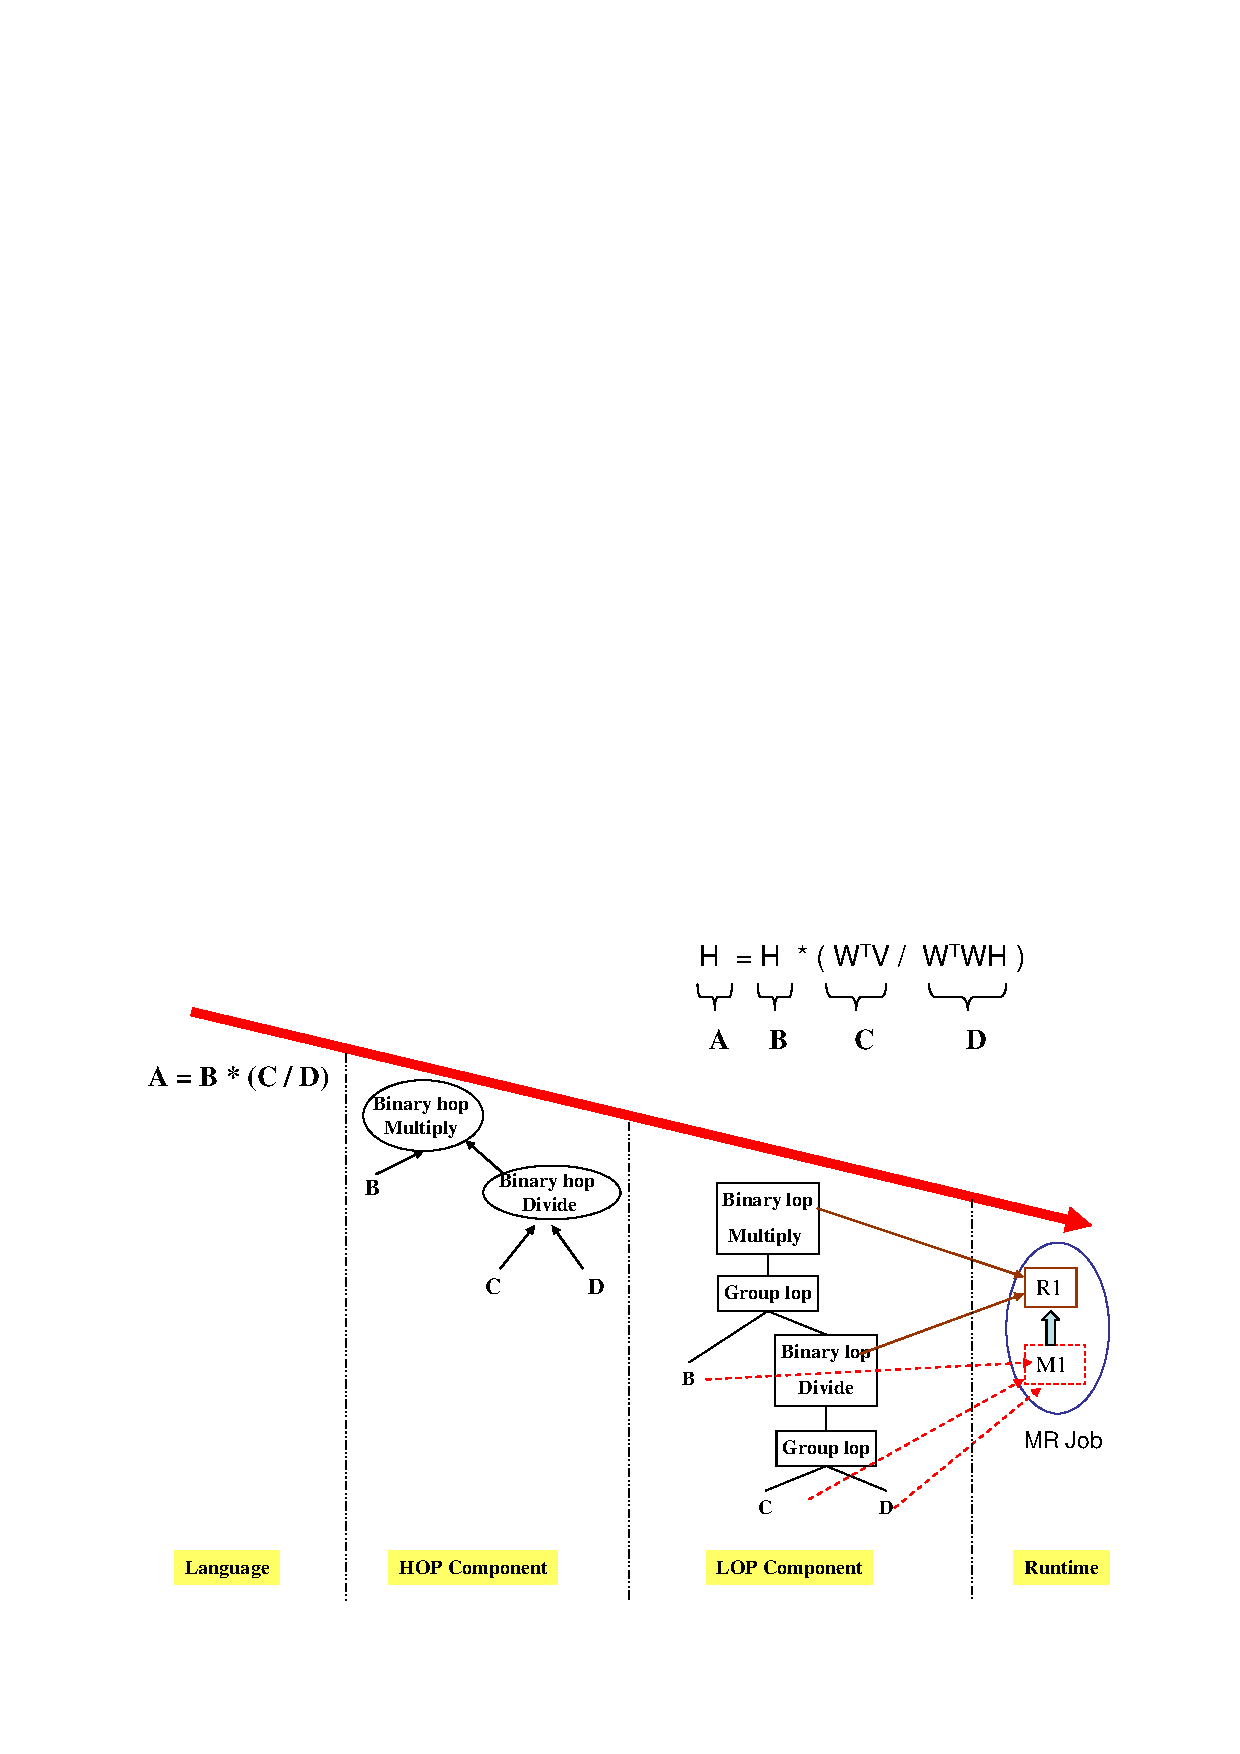
\includegraphics[width=3.7in]{example.pdf}
\caption{(a) Illustrating submatrix partitioning. The grey portion
corresponds to $A$, yellow corresponds to $B$, blue corresponds to $C$ and the
red portion corresponds to the $D$ matrix. (b) When the partitioning boundary
aligns with the block boundaries. Each small rectange indicates a block.
(c) Case when the block boundaries do not align
with the partition boundary.}
\label{fig:submatrixmove}
\end{figure}
}

\subsection{Cell Partitioning}
\label{sec:cell-part}
We now describe the split generation method for cell granularity in Table~\ref{?}, which 
is used to support Wold Holdouts for CV. 
In this approach, we randomly holdout a small fraction of the cells in the matrix for a test set, and the remaining are used for training.
The challenge in correctly implementing cell partitioning for sparse matrices is that only non-zero elements in the matrix are explicitly stored.  Hence, directly iterating over the non-zero matrix cells would not lead to an uniform partitioning.
Instead, we generate bit matrices corresponding to the held out portion of the matrix.
For each iteration, we create a bit matrix $B$ with entries either $0$ or $1$. 
If $B_{ij} = 1$, then the corresponding cell in the given data matrix $A$ is held out 
(i.e., test dataset), otherwise, the entry is held in (i.e., in the train dataset).
%Note that the training algorithm using cell-based partitioning needs to be written 
%based on these bit matrices.
\cite{nips2010} describe efficient strategies to learn {\em weighted NMF} models using such bit matrices.

\section{Cost-based Optimization for Split Generation}
\label{sec:optimization}

This section describes how SystemML selects the appropriate plan for evaluating the declarative
CV and EL operators from the space of possible plans.
The UDFs implementing training (model building), testing (using ensemble),
and error aggregation (prediction combination) in CV (EL) are already optimized by SystemML.

Thus, this section focuses on selecting the most efficient method for the {\tt GENSPLITS} task from the available methods and the scheduling of tasks to evaluate the CV and EL operators (i.e., {\tt GENSPLITS}, the UDFs for training, test, and error aggregation).

In Section~\ref{sec:rowpartitioning}, we propose three possible implementations of
row-based split generation. To determine the most efficient method at runtime, we develop a cost model based on the data and system characteristics most influencing the performance of these methods. Thus, SystemML can use the cost model to automatically select at runtime the most efficient method.

The costs for the three row-based split generation algorithms described in
Section~\ref{sec:rowpartitioning} are shown in Figure~\ref{fig:costmodel}.
We measure the I/O cost in terms of total number of bytes,
and for shuffling in terms of both total number of bytes and number
of key-value pairs that flow through the jobs.
As we can see from the table, there is no clear winner among the three approaches in all cases.
The HashMap (HM) approach has the lowest shuffle costs in most cases; however,
it has a significant I/O cost since the map table needs to be read by each of
the mappers (distribution costs). Furthermore, HM is limited
by the memory size in each mapper (i.e., the HashMap of size $8mk$ bytes must fit into the memory of the mapper,
where $m$ is the number of rows and $k$ is the number of folds / ensemble models).
Overall, the Reblock (RB) approach has the highest costs in most cases (for large-scale data, usually
$m,n >> k, P$), with the Join-Reblock (JR) method having performance between the RB and HM.
Either the HM or JR approach is required for RSM and
sampling with replacement, with the JR method not having the memory limitation of HM.

We currently use the following approach for the optimizer to pick the method.
We check if the hashmap for HM can fit in the memory of each mapper; if so, we use the HM strategy.
Otherwise, we compute the shuffle costs for JR and RB methods and select the
method with the smaller shuffle cost. If the shuffle costs are are comparable,
we use the method with the smaller I/O cost. As we see later in the experiments,
for the datasets we considered, the optimizer usually picks the HM method due to large
available memory.
However, if memory on each mapper is limited, the optimizer typically picks JR,
as suggested by the cost formulae.
Our experimental evaluation in the next section validates the cost model captures
the characteristics which dominate the performance of split generation.
For submatrix partitioning (Section~\ref{sec:submatrix}), we showed the block-based method is more efficient for all datasets and
only a single method for cell partitioning was presented in Section~\ref{sec:cell-part}.

\topicnoul{Scheduling}: Since we know the exact semantics for CV and EL
(i.e., split generation, multiple training and model evaluation), we can
effectively parallelize and schedule computation as necessary.
As described, the {\tt GENSPLITS} operator constructs all splits by replicating
the dataset for each fold or ensemble model training set. However, this may
not be feasible in practice, especially when considering very large-scale
10000-fold cross-validation or ensembles with thousands of models.
To support this case, we make a straightforward modification to {\tt GENSPLITS} to only
generate per execution as many folds as feasible, based on available storage on the HDFS.
Similarly, SystemML can evaluate in parallel multiple folds for CV and EL.
Each CV fold produces two UDF calls, a training function call
and testing function call. Since the CV folds are independent, an arbitrary
number of these UDFs can be scheduled in parallel based on available system resources.
After all folds are evaluated, the final error aggregation UDF is invoked.
EL is parallelized in a similar manner, since the construction of each ensemble model is independent.

\section{Implementation Details}
\label{sec:implementation}

We briefly mention other relevant implementation details for the CV and EL language operators.

\topic{Runtime compilation:}\\
In addition to the DML language constructs, we introduced additional HOPs and LOPs to support CV and EL.
We compile and optimize the train and test user-defined functions at runtime, for each fold or ensemble model after
obtaining the sizes of the matrices resulting from the {\tt GENSPLITS} step. The overhead of repeated compilation
is negligible (milliseconds) relative to function execution time.

\topic{Pseudo random sampling on Hadoop}\\
SystemML uses random sampling to compute the various folds for cross-validation.
Since SystemML is based on a parallel platform Hadoop, care must be taken to
ensure that the random sampling is unbiased and perfectly pseudo random.
For this purpose, we use {\tt WELL1024}~\cite{L'Ecuyer:1990:RNS:84537.84555}, a
long period random number generator (PRNG) with period of approximately $2^{1000}$.
Each period can be split into $2^{300}$ streams each of length $2^{700}$, and efficient skipping over substreams is supported as well.
We incorporate WELL1024 PRNG into SystemML as follows.
Each mapper is assigned a unique identifier and a particular number of substreams based on the type
of partitioning required. For example, suppose that each mapper requires 2 streams (k-fold stratified
cv with domain size = 2). In that case, if we get to the mapper with id = 4, we first skip 6 times to
get the first stream for the mapper and skip again to get the second stream for the mapper.
Experimental results indicate the time taken for such skipping is typically subsecond for over 10,000 substreams.

\topic{Supporting Stratification} \\
As mentioned in Section~\ref{sec:background}, supervised learning tasks require
the folds to be stratified based on the class label. We support
stratification for row-based partitioning tasks using multiple seeds. We
illustrate with an example. Suppose that we want to classify emails as spam or
genuine. In this case, we use $2$ seeds, one for each email type. For each row,
we examine its class label and sample from the appropriate seed.


\section{Experiments}
\label{sec:experiment}
The experimental evaluation in Section~\ref{sec:experiment} demonstrates that HM and JR approaches are faster
than RB for partitioning and sampling without replacement for a wide range of input data characteristics.

The goal of our experiments is to study the performance and scalability of the
various algorithms for data partitioning under different data and system characteristics.

\paragraph*{Experimental Setup}
The experiments were conducted with Hadoop 0.20 on a 40-core cluster with 5 local
machines as worker nodes. Each machine has 8 cores with hyper-threading, 32 GB RAM
and 2 TB storage. We set each node to run XX concurrent mappers and XX concurrent
reducers. The datasets are synthetic, and for given dimensionality
and sparsity, the data generator creates random matrices with
uniformly distributed non-zero cells. A matrix block size of 1000 $\times$ 1000 is used.

\subsection{Row Partitioning}
We first compare the performance and scalability of the three row partitioning
schemes -- Reblock-Based (RB), Join-Reblock (JR) and HashMap (HM). We vary the
input matrix characteristics, viz., number of rows, number of columns and sparsity,
fixing two at a time, as well as the number of folds.

\paragraph*{Number of Rows}
Figure \ref{fig:row:row} plots
the runtimes for $k$-fold CV and bagging EL against the number of rows. The number of
columns is fixed at 10000 with sparsity at 0.1\% and 5 output folds. The fraction
(relative size of train fold) for bagging is 0.3.
We see that all three methods (RB, JR and HM) scale linearly with the number of rows.
As expected, HM performs the fastest (nearly 3x faster than RB), and JR is only slightly
faster than RB. However, it should be noted that as the number of rows goes up, HM will
eventually crash due to insufficient memory, while JR and RB continue to scale. Also,
RB is not applicable to bagging since it involves with replacement sampling as explained
in Section \ref{sec:rowpartitioning}.

\begin{figure}[h]
\centering
\includegraphics[width=1.64in]{row/row-cv.pdf}
\includegraphics[width=1.64in]{row/row-el.pdf}
\caption{Performance of Row-partitioning schemes: (a) $k$-fold CV (b) Bagging EL against
number of rows}
\label{fig:row:row}
\end{figure}

\begin{figure}[h]
\centering
\includegraphics[width=1.64in]{row/col-cv.pdf}
\includegraphics[width=1.64in]{row/col-el.pdf}
\caption{Performance of Row-partitioning schemes: (a) $k$-fold CV (b) RSM EL against
number of columns}
\label{fig:row:column}
\end{figure}

\paragraph*{Number of Columns}
Figure \ref{fig:row:column} plots
the runtimes for $k$-fold CV and RSM EL (which partitions on columns)
against the number of columns, fixing
the number of rows at 1 million and sparsity at 0.1\%. The number of folds is
again 5 and the fraction for RSM is set at 30\%. Again, we see a linear scaleup
for all methods, but JR performs almost the same as RB as number of columns
goes higher. This is because the reduce-side join becomes more CPU-intensive
owing to the larger row sizes. Again, RB doesn't handle RSM as explained in
Section \ref{sec:rowpartitioning}.

\paragraph*{Sparsity}
Figure \ref{fig:row:sparsity:fold} (a) plots
the runtimes for holdout EL against the sparsity of the input matrix, fixing the other
variables. Since the number of cells that flow in the MapReduce jobs is linearly dependent
on the sparsity, we see that all the methods scale linearly with sparsity.

\paragraph*{Folds}
Figure \ref{fig:row:sparsity:fold} (b) plots
the runtimes for Holdout CV against the number of folds, fixing the other variables. Again,
as expected, we see a linear increase in the runtime for all the three methods.

\begin{figure}[h]
\centering
\includegraphics[width=1.64in]{row/sparsity.pdf}
\includegraphics[width=1.64in]{row/fold-cv.pdf}
\caption{Performance of Row-partitioning schemes: (a) Holdout EL against sparsity (b) Holdout
CV against number of folds}
\label{fig:row:sparsity:fold}
\end{figure}

\subsection{Submatrix Partitioning}
Next, we compare the performance of the two submatrix partitioning schemes -- Cell-Based (P1)
and Block-Based (P2). In this experiment, we illustrate the advantages of
blocking the input matrix for submatrix partitioning. We start with a matrix in
cell format and partition it using two different plans. In the first approach P1, we
execute $2\times 2$ partitioning using the cell-based approach
(Section~\ref{sec:submatrix}. In the second approach P2, we use a two step process in which we
initially block the matrix using a reblock job and subsequently use the
block approach for partitioning. We measure the time taken for each case. For
the second case, we compute the time taken for both the reblocking and the
partitioning. The results are shown in \ref{fig:submatrix} (a). We execute
two experiments with different column sizes. In each experiment, we vary the
number of rows in the matrix.
As shown in the figure, the time taken in $P_2$ is much less than $P_1$. We
would like to note here that this may seem counter intuitive
since we are actually making two passes over the data. The reason for this is
that in the first case, we are replicating cells (while shuffling) where as in
the second case we are only replicating blocks, which are much fewer in number.

\begin{figure}[h]
\centering
\includegraphics[angle=-90,width=1.64in]{optimization.pdf}
\caption{Performance of submatrix-partitioning schemes}
\label{fig:submatrix}
\end{figure}

\subsection{Speed-up and Scale-up}
Here, we study the speed-up and scale-up behavior of the row partitioning methods.
We plot the runtimes against the number of reducers in
Figure \ref{fig:speedup:scaleup}(a). We then vary the dataset size proportional
to the number of reducers and plot the runtimes in Figure \ref{fig:speedup:scaleup} (B).
We (should) see that the speed-up is linear as we increase the number of reducers.
However, the scale-up is not flat since there will be more network overheads as the
number of reducers increases.

\begin{figure}[h]
\centering
\caption{Speedup and Scaleup: TODO}
\label{fig:speedup:scaleup}
\end{figure}


\eat{
\section{Experimental Evaluation}
\label{sec:experiment}

We start with a description of the experimental setup and the main objectives
of our analysis.

\subsection{Objectives}
The main objectives of our experimental analysis are as follows.
\begin{enumerate}
\item {\em Necessity of a declarative system for large-scale meta-learning:}
Here, we compare the performance of the proposed algorithms for row partitioning
for various matrix characteristics.
\item {\em Scale-up of partitioning jobs:} Here, we demonstrate the {\em
scale-up} and {\em speed-up} of the partitioning jobs for rows and sub-matrices.
\item {\em Illustrating advantages of optimization \& scheduling}
\end{enumerate}

\subsection{Results}
\topic{Necessity of a declarative system for large-scale machine learning} \\
We consider different matrix characteristics $C_1$, $C_2$ and $C_3$ as defined
below and execute different algorithms for row partitioning over them
(Section~\ref{sec:design}). We denote $P_1$ to be the method using
reblock. $P_2$ is the method using hashmap and $P_3$ to be the method using
joins.
\begin{enumerate}
\item $C_1$: {\em Number of rows:} For small number of rows, we see that $P_2$
is the best method since the hash map fits in memory. As we increase the number
of rows, the reblock method wins since we cannot maintain hashmap in memory.
When we increase the number of rows further, the join method ultimately beats
out the remaining methods. Note that this is in spite of join method using both
map and reduce phases.
\item $C_2$: {\em Number of columns} Here, we plot the performance of our row
partitioning algorithms over matrices with different number of columns. As we
can see from the plots, when the number of columns is low, the reblock method
works well. However, when the number of columns is very large, the row block may
not fit in memory and the join method works well.
\item $C_3$ {\em Number of non-zeros} Here, we fix the number of rows and
columns in the matrix and gradually increase the number of non-zero elements in
the matrix. As expected, we find that its behavior is similar to increase the
number of columns in the matrix.
\end{enumerate}

As shown by the above figures, there is no clear winner among the three methods
and the matrix characteristics dictate the best approach for partitioning. Given
the large number of factors involved, a declarative system is essential for
scaling large-scale cross-validation and ensemble learning tasks.

\topic{Scalability of partitioning jobs:} \\
Here, we demonstrate the scale-up and speed-up of the partitioning
algorithms. We run the following experiments.

\begin{enumerate}
\item {\em Speed-up:} We carry out two experiments here. In the first
experiment, we increase the number of mappers and measure the total speedup
obtained for the row partitioning and the matrix partitioning algorithms. In the
second experiment, we increase both the number of mappers and reducers and
measure the speedup obtained. We notice here that the speedup in the second
experiment is almost equal to the speedup obtianed in the first experiment. This
is because the number of reducers actually used by Hadoop is equal to the number
of files written (e.g., for $k$-fold cross-validation it is $2k$).

\item {\em Scale-up:} Here, we carry out the following experiments. In the first
experiment, we increase the number of rows and simultaneously increase the
number of mappers \& reducers to measure the time taken for row-based k-fold
cross-validation. Next, we repeat the experiment by increasing the column size
of the matrix. Following this, we execute the above experiments for the case of
sub-matrix partitioning.

\item {\em Increasing number of folds} We carry out two experiments here. In the
first experiment, we execute row-based k-fold cross-validation with different values of
$k = 5, 10, 15$. As shown in Figure~\ref{fig:results}(f), as we increase the
number of folds, the amount of time taken increases linearly.

\item {\em Submatrix scalability} In this experiment, we measure the scalability
of the submatrix partitioning jobs. In Figure~\ref{fig:results}(g), we measure
the scalability of the cell-based partitioning jobs. As we increase the number
of rows in the matrix, we obtain a close to linear increase the computation
time. However, the slope is dependent on the number of columns in the matrix. In
Figure~\ref{fig:results}(h), we perform the same experiment on the block-based
partitioning job and obtain similar results.
\end{enumerate}


\begin{figure*}
\begin{tabular}{ccc}
%\includegraphics[width=2.5in]{time.pdf} &
%\includegraphics[width=2.5in]{time2.pdf} &
%\includegraphics[width=2.5in]{kfold.pdf} \\
%(a) & (b) Row partitioning & (c) Linearly increases in $k$ \\

\begin{minipage}{2.3in}
\begin{tabular}{|c|ccc|}
\hline
&Reblock& Hashmap& Join \\
\hline
Case 1 &&&\\
Case 2 &&&\\
Case 3 &&&\\
Case 4 &&&\\
Case 5 &&&\\
\hline
\end{tabular}
\end{minipage} &
\hspace*{-0.2in}
\begin{minipage}{2.3in}
\includegraphics[angle=-90,width=2.3in]{blank.pdf}
\end{minipage} &
\hspace*{-0.2in}
\begin{minipage}{2.3in}
\includegraphics[angle=-90,width=2.3in]{blank.pdf}
\end{minipage} \\
(a) Declarative & (b) Scaleup (Row) & (c) Scaleup (Row) \\

\includegraphics[angle=-90,width=2.3in]{blank.pdf} &
\hspace*{-0.2in}
\includegraphics[angle=-90,width=2.3in]{blank.pdf} &
\hspace*{-0.2in}
\includegraphics[angle=-90,width=2.3in]{kfold.pdf} \\
(d) Speedup (Row) & (e) Speedup (Row) & (f) Scalability (folds) \\


\includegraphics[angle=-90,width=2.3in]{submatrix-cell.pdf} &
\hspace*{-0.2in}
\includegraphics[angle=-90,width=2.3in]{all-block.pdf} &
\hspace*{-0.2in}
\includegraphics[angle=-90,width=2.3in]{optimization.pdf} \\
(g) Scalability Submatrix (cell) & (h) Scalability Submatrix (block) & (i) Optimization \\


\includegraphics[angle=-90,width=2.3in]{blank.pdf} &
\hspace*{-0.2in}
\includegraphics[angle=-90,width=2.3in]{blank.pdf} &
\hspace*{-0.2in}
\includegraphics[angle=-90,width=2.3in]{blank.pdf} \\
(j) Scheduling (concat) & (k) Scalability CV (NMF) & (l) Scalability CV (LR) \\

\end{tabular}

\caption{Experimental Results}
\label{fig:results}
\end{figure*}

\topic{Optimization}

\begin{itemize}
\item {\em Blocking for submatrix partitioning:}
In this experiment, we illustrate the advantages of
blocking the input matrix for submatrix partitioning. We start with a matrix in
cell format and partition it using two different plans. In the first plan $P_1$, we
execute $2\times 2$ partitioning using the cell-based approach
(Section~\ref{sec:}. In the second plan $P_2$, we use a two step process in which we
initially block the matrix using a reblock job and subsequently use the
block approach for partitioning. We measure the time taken for each case. For
the second case, we compute the time taken for both the reblocking and the
partitioning. The results are shown in Figure~\ref{fig:results}(i). We execute
two experiments with different column sizes. In each experiment, we vary the
number of rows in the matrix.
As shown in the figure, the time taken in $P_2$ is much less than $P_1$. We
would like to note here that this may seem counter intuitive
since we are actually making two passes over the data. The reason for this is
that in the first case, we are replicating cells (while shuffling) where as in
the second case we are only replicating blocks, which are much fewer in number.
\end{itemize}


\topic{\em Scheduling:}\\ This allows us to replace the partition operator
with multiple concat operators, essentially creating a HOPS/LOPS dag which is
disconnected. This allows us to start training on the 1st fold, while the second
fold is being constructed. Note that this scheduling must be aware of the amount
of disk space that is available on the HDFS. While learning, we consume the
folds and can create additional space for subsequent folds. I am planning to
test the three approaches (measure make-span: time for entire task to complete)
\begin{enumerate}
\item Construct all folds at once. The graph will essentially show that for
$k=10$ and above, Hadoop will throw I/O errors due to lack of space. Space is
the biggest constraint for large-scale.
\item One-by-one: This is the other extreme when we learn the fold, then build
the next fold and so on.
\item Our scheduling: Intelligently schedule jobs by making use of available
resources.
\end{enumerate}
}

\section{Related work}
\label{sec:related}

Large-scale machine learning has become an important research task given the \emph{application pull} --
spam detection, personalized search, recommendation
application etc. and {\em technology push} -- availability of large-scale data processing
tools such as MapReduce and multicore systems.
Examples of such systems include Apache Mahout~\cite{mahout}, Google prediction API~\cite{gapi},
SystemML~\cite{systemml}, GraphLab~\cite{Low+al:uai10graphlab}, Pegasus~\cite{DBLP:conf/icdm/KangTF09},
Spark~\cite{spark}, and DryadLINQ~\cite{dryadLINQ}. Further, there has been a great deal
lot of literature including \cite{DBLP:conf/nips/ChuKLYBNO06,DBLP:journals/pvldb/CohenDDHW09}.
Our work extends one of this large scale machine learning systems, SystemML,
to support cross-validation and ensemble learning as a first-class declarative operator.

Sections~\ref{sec:cvbackground} and \ref{sec:elbackground} provide background on cross-validation and ensemble learning. Typically, a standalone package will support CV or EL for a particular machine learning technique. E.g., the {\tt randomforest} package in R implements random forest ensembles for decision trees. Approaches to parallelize CV and EL in a MapReduce setting typically address a single technique as well. \cite{parallel-boosting} parallelizes AdaBoost and LogitBoost for ensembles, while PLANET \cite{planet} builds ensembles of {\em decision trees} over very large scale data using MapReduce.
In contrast, we develop declarative operators for generic meta learning for all kinds of models and ensemble techniques. Our approach can efficiently support both the parallel boosting in \cite{parallel-boosting} and random forests, along with CV and EL for many other kinds of models.

\section{Conclusions}
\label{sec:conclusions}
Massive amounts of data generated on the web are used to routinely train very
complex machine learning models for solving a range of problems such as spam
detection, recommender systems, personalized search and advertising.
Consequently, verifying the quality of machine learned models has become an
important task. Cross-validation is a versatile tool that has been extensively
used for solving this problem, as well as a number of related problems such as
model-selection and feature selection.
In this paper, we build a system that provides the ability to cross-validate
all possible machine learning models
(including unsupervised models) over very large-scale datasets using the
MapReduce framework. As we show in the paper, owing to the multitude of methods
to cross-validate a given machine learning model (for e.g., partitioning
techniques) and the various potential implementation strategies, we need to
develop a declarative system that can choose the best possible plan for a given
cross-validation task. In future, we intend to extend our system for performing
other meta-learning tasks such as boosting, stacking and other ensemble
strategies. We also plan to develop scalable cross-validation strategies for non
i.i.d samples such as relational learning models.

\bibliographystyle{abbrv}
{
\small
\bibliography{internreport}}

\end{document}
